\documentclass{article}



\usepackage{arxiv}

\usepackage[utf8]{inputenc} % allow utf-8 input
\usepackage[T1]{fontenc}    % use 8-bit T1 fonts
\usepackage{hyperref}       % hyperlinks
\usepackage{url}            % simple URL typesetting
\usepackage{booktabs}       % professional-quality tables
\usepackage{amsfonts}       % blackboard math symbols
\usepackage{nicefrac}       % compact symbols for 1/2, etc.
\usepackage{microtype}      % microtypography
\usepackage{lipsum}		% Can be removed after putting your text content
% \usepackage{xcolor}
\usepackage[table,xcdraw]{xcolor}
\usepackage{graphicx}
\usepackage{float}


\definecolor{codegray}{gray}{0.9}
\newcommand{\code}[1]{\colorbox{codegray}{\texttt{#1}}}


\definecolor{ironmancolor}{rgb}{0.9, 0.4, 0.38}
\newcommand{\ironman}[1]{\colorbox{ironmancolor}{\texttt{#1}}}



\title{Avengers EndGame: \emph{friday, let's save the universe!}}

% \date{October 31, 2019}	% Here you can change the date presented in the paper title
%\date{} 					% Or removing it

\author{
  Amr M.~Kayid\\
  Department of Computer Science\\
  German University in Cairo\\
  Cairo, Egypt 11841 \\
  \texttt{amrmkayid@gmail.com} \\
  %% examples of more authors
   \And
 Ahmed A.~Fathy \\
 Department of Computer Science\\
 German University in Cairo\\
 Cairo, Egypt 11841 \\
  \texttt{ahmedadelfathy97@gmail.com} \\
    \And
  Ahmed A. Bayoomi \\
  Department of Computer Science\\
  German University in Cairo\\
  Cairo, Egypt 11841 \\
  \texttt{ahmedamb2214@gmail.com} \\
  %% \And
  %% Coauthor \\
  %% Affiliation \\
  %% Address \\
  %% \texttt{email} \\
  %% \And
  %% Coauthor \\
  %% Affiliation \\
  %% Address \\
  %% \texttt{email} \\
}

% Uncomment to remove the date
%\date{}

% Uncomment to override  the `A preprint' in the header
%\renewcommand{\headeright}{Technical Report}
%\renewcommand{\undertitle}{Technical Report}

\begin{document}
\maketitle

\begin{abstract}
  In attempt to save the universe, Iron Man has build a new advanced suite (\textit{Mark 700}) which is going to help him searching for the infinity stones to collect them, defeat thanos' warriors (\textit{Thanos' Sons}) and beat Thanos by snapping his finger to return the universe to the way it was used to be. Friday (\textit{Iron Man's Advanced A.I.}) is going to find the best possible strategies to help iron man in saving the universe. Friday will be using advanced ai search algorithms (\textit{e.g. A* Search}), consult some logical agents and running millions of simulations inside her brain to come up with the best and most efficient way for iron man to defeat thanos and save our lovely universe.
% \lipsum[1]
\end{abstract}


% keywords can be removed
\keywords{Artificial Intelligence\footnote{This paper is associated as a part of research project within GUC CSEN 901 Introduction to Artificial Intelligence Course~\cite{csen901}} \and Generic Search Algorithms \and Logic Agents \and Unity ML Agents \and Reinforcement Learning}


\section{Introduction}
In this research project, we are creating a new environment which will be suitable for designing and testing intelligent different types of agents. The aim of this research paper is to introduce the new environment and demonstrate the different kinds of agents that solve the environment and provide comparisons between them while benchmarking the performance and efficiency for each type. Finally we conclude our experiments and discuss the future work.

We are going to design the new environment in a generic way which can be extended to different types of platforms. A brief introduction to our environment and the problem we are trying to solve using intelligent agent is introduced in the following paragraph. 

The new environment \textbf{(End Game)} is represented as a 2D grid \textit{(universe)} of cells consisting of \textbf{m rows} and \textbf{n columns} (\textit{where 5 $\leq$ m,n $\leq$ 15}). A grid cell is either \textit{free} or contains one of the following: \textit{iron man}, \textit{thanos}, one of Thanos’ \textit{warriors}, or an \textit{infinity stone}. In this project, we will use generic search algorithms to help Iron Man defeat Thanos by first collecting the six infinity stones, then heading to the cell where Thanos is frozen, and finally snapping his fingers to return the universe to the way it used to be and vanish thanos world. Iron Man can move in the four directions as long as the cell in the direction of movement does not contain Thanos or a living warrior. He can collect an infinity stone only if he is in the same cell with the stone. Since the stones possess immense powers, collecting a stone causes \textbf{3 units} of damage to Iron Man. At any point with one move, Iron Man can kill all warriors lying in adjacent cells. An adjacent cell is a cell that lies one step to the \textit{north, south, east, or west}. Killing a single warrior will increase Iron Man’s received damage by \textbf{2 units} since they will attempt to fight back. Once a warrior is killed, Iron Man can move through the cell where the warrior was. 

Since Thanos and his warriors are very powerful, they can cause damage to Iron Man as long as he is in an adjacent cell to them. Being in an adjacent cell to Thanos increases Iron Man’s received damage by \textbf{5 units} for each time step, while being in an adjacent cell to a warrior increases Iron Man’s received damage by \textbf{1 unit} for each time step. A time step is the time required to do an action. After collecting the stones, Iron Man will be able to enter the cell where Thanos is and snap his fingers only if \textit{his received damage is less than \textbf{100 units}}.

% This project is designed in a way that combine search algorithms design along with reinforcement learning designs and styles in a way for comparing between both and seeing the performance of the agents.

% \clearpage

\section{Architecture}
\label{sec:architecture}

% See Section \ref{sec:architecture}.
In this section, we will discuss the architecture used to design the problem by following the best practices found through ~\cite{aimajava, aimapython} and the techniques and strategies used to solve the problem. 
% TODO: describe LBA & RL archs

\subsection{EndGame State}
The environment observations is designed through an abstract class \textit{State} for representing the state of the environment after each time-step. \textit{EndGameState} is a subclass from our abstract class which is a 5-tuple contains the following:
\begin{itemize}
  \item \textbf{Iron Man Position}: This is a pair of \textit{<row, col>} integers that represent the current location of iron man in the universe grid.
	\item \textbf{Iron Man Damage}: the current received damage of iron main. Initially equals to zero.
	\item \textbf{isThanosDead}: Boolean variable to test whether thanos is dead or not which is used for the goal test.
	\item \textbf{Infinity Stones}: A set of pairs containing the location of each infinity stone in the universe.
	\item \textbf{Warriors Positions}: A set of pairs containing the location of each warrior in the universe.
\end{itemize}

\subsection{Search Node}
% TODO: Check Cite
Following Russell and Norvig design approach~\cite{russell2016artificial}, we consider search node to be 5-tuples containing:
\begin{itemize}
  \item \textbf{State}: the current state of the state space that this node corresponds to.
  \item \textbf{Parent node}: the node that leads to the current node after applying the action
  \item \textbf{Action}: the action applied to generate this node.
  \item \textbf{Depth}: the depth of the node in the tree.
  \item \textbf{Path Cost}: the path cost from the root.  
\end{itemize}

\subsection{Search Problem \textit{(BaseEnv)}}
The design of the search problem is based on the concept of environment in which we have a list of actions that can be performed by the agent and the environment gives us updates for it's current state and the next state that will be generated after applying any action from the agent. This is summarized in the following variables \& methods:
\begin{itemize}
  \item \textbf{Actions}: List of actions objects available to the agent.
\item \textbf{Initial State}: An \textit{EndGameState} object representing the initial state of the search agent. This gets generated from \code{reset()} method.
\item \textbf{State Space}: Using a method called \code{step()} that takes a \code{\textit{State}} object and an \code{\textit{action}} object and returns a \code{\textit{State}} object after applying the action to the input state.
\item \textbf{Goal Test}: A method that checks whether a state is a goal state or not.
\item \textbf{Path Cost} A method that takes \code{\textit{node}} object and an \code{\textit{action}} object and calculates the path cost value of this particular node.
\end{itemize}

\subsection{EndGame Environment}
Our main environment for the project is the \code{\textit{EndGame}} environment class. This is responsible for initializing a singleton instance from \textit{EndGameUniverse} which is a 2D grid representation for the \textit{environment} from the given \textit{gridString} input. In the following subsections, we describe the properties and methods used inside EndGame class for searching and solving the given problem.
\subsubsection{Initial State}
Using the initialized universe, the environment instantiate the initial state \textit{(EndGameState instance object)} which is accessible through \code{reset()} method. This state contains the initial position for iron man, initializing the damage to equal zero, contains a \textit{set} of positions for both infinity stones and warriors.

\subsubsection{Actions}
An implemented abstract \code{Action} class is introduced for representing the actions available for the agent inside the environment. After that, we implemented \code{EndGameAction} subclass which is a generic representation for all the actions in \textit{EndGame} environment class. This class implement the methods responsible for checking the validation for movement actions, getting the adjacent cells for a given input cell in a particular state, checking for warriors at a given state and computing the damage that \textit{iron man} could get after each time step in the environment. In the following subsections we describe the functionality of each action:

\begin{itemize}
  \item \textbf{Movement Action}: This class is responsible for the movement of our agent \textit{(iron man)} inside the universe. The available movement actions are \textit{(Up, Down, Left, Right)}, where iron man can move freely inside the universe as long as the movement is valid and does not cross the border of the universe and also the cell is free (e.g. does not contain warrior or thanos). before performing the movement, we check for the damage that can happen from being in an adjacent cell to warrior or thanos which increase the damage by 1, or 3 respectively. For handling repeated states, we check if the new state does not match the same state from the parent which can happen when undoing, redoing the same action again.

  \item \textbf{Collect Action}: This class is responsible for enabling our agent \textit{(iron man)} to collect one of the \textit{infinity stones} in the universe. Since the stones possess immense powers, collecting a stone causes \textit{3 units} of damage to Iron Man. we also check for the damage that can happen from being in an adjacent cell to warrior or thanos which increase the damage by 1, or 3 respectively. After collecting the stone, it gets removed from the set of available stones in the universe and a new state is returned inside a new generated node.

  \item \textbf{Kill Action}: This class is gives our agent \textit{(iron man)} the ability to kill the warriors inside the universe. Hence, Iron Man can kill all warriors lying in adjacent cells. An adjacent cell is a cell that lies one step to the north, south, east, or west. Killing a single warrior will increase Iron Man’s received damage by \textit{2 units} since they will attempt to fight back. Once a warrior is killed, Iron Man can move through the cell where the warrior was. After killing the warriors, they get removed from the warriors set and a new state is returned inside a new generated node.

  % TODO: Remove and organize actions =<>= GRID

  \item \textbf{Snap Action}: The is the super action that solves the environment and return universe's eliminated half by reversing what Thanos did and kill Thanos once and for all. This action can only be performed only if \textit{iron man} damage is less that \textit{100 unit} and he is in the same position as thanos and most importantly \textit{iron man} should have collected all the six stones in the universe and snapping his finger saying \ironman{\textbf{\textit{"I AM IRON MAN!"}}}\footnote{I am super attached to the movie :)) | to be removed}.

\end{itemize}


\subsection{State Space}
State space is represented in the transition function \code{step()} which is used to get the next state after applying a given \textit{action} on the \textit{current state} of the environment. For the search problem algorithm, we use \code{expand(Node node)} method which initially takes the initial node containing the initial state of the environment and start checking for each action that the agent can use to act upon the state in the environment and expand the current node to a list of available not after the agent acting using the valid actions in the current state. This method gets called inside the search algorithm and keep expanding the search tree till ending up at a goal state and solving the environment problem.


\section{Methods}
In the following figure~\ref{fig:flow}, a summary for the flow of the whole project for search agents and how they interact with the environment.

% TODO: Update the figure 
% => current node arrow to the expand fn.
\begin{figure}[!hpt]
  \centering
  \includegraphics[width=\linewidth]{figures/EndGame.png}
  \caption{The project main functionally and flow of the program}
  \label{fig:flow}
\end{figure}

As shown in the figure, the flow of the program starts by initializing an instance of the universe map given the \textit{gridString} input. After that, we reset the environment and return the initial state of the universe containing all the details required for the agents and search tree to solve the problem. This state is turned to the initial node and get sent to the \textit{BaseAgent} which is the super class for all search strategies. This is followed by calling the \code{search} method which iteratively \textit{sample} the next node to be explored from the agent, check whether or not it is a goal test, then expand the tree till finding the goal state or finding no solution if the agent's buffer gets empty. Upon founding a solution, an output string is returned and either visualizing the steps that leads to the solution or terminate the program and close the environment.

\subsection{Generic Search Algorithms}

The implementation of the search algorithms are based on the concept of agent. Hence, we have implemented an abstract \code{BaseAgent} class that represent \textbf{the brain} of the agent which include the \textit{initial state} of the environment and a \textit{memory} that is used for storing the previous states and compare between the new add states in the agent brain. Following a set of various search algorithms that inherit from the \textit{BaseAgent} class and implement the different strategies for searching in the environment.

\subsubsection{Breadth-first Search (BFS)}\label{bfs}
Breadth-first search explores the search tree \textit{level by level}. This is done by implementing \textit{first in first out} (FIFO) data structure where we add the new expanded nodes are the end of the buffer. Hence, for BFS we will be using java \textit{queue} to store the explored search tree nodes. In the \textit{BreadthFirst} class, the initialized buffer is represented as a \textit{Java Queue}. We add nodes in the buffer using \code{add()} methods, and when removing a node from the queue using \code{sample()} method for exploring and expansion we first check whether it’s visited or not to \textit{prevent repeated states}. Then, the state is saved in the agent's memory and a new node is returned.

\subsubsection{Depth-first Search (DFS)}\label{dfs}
Depth-first search explores the search tree by selecting a single path, reaches the end of the path \textit{(leaf node)} then backtracking to another path until it finds the solution node. This is done by implementing \textit{last in first out} (LIFO) data structure. This implies using java \textit{stack} for representing the buffer used in the DepthFirst class. The process of adding and sampling states from the buffer is the same as in (BFS)~\ref{bfs}. The design of this class contains property of \textit{limit} which correspond to the max depth limit that will be useful when implementing iterative deepening search algorithm described in the next Section~\ref{ids}.
\subsubsection{Iterative Deepening Search (IDS)}\label{ids}
Iterative deepening search (or iterative deepening \textit{depth-first search}) is a general strategy, often used in combination with depth-first tree search, that finds the best depth limit. It does this by gradually increasing the \textit{limit} first 0, then 1, then 2, and so on until a goal is found. This class uses an instance from DFS~\ref{dfs} where the difference is in sampling nodes and checking the emptiness of the buffer. The process is that when sampling, we check not only it's a repeated state in the memory but also using the \textit{limit} property we check the current depth of the node and whether the node exceeds the limit, thus it is not valid. This process continues until the buffer gets empty in which case we increase the limit by \textbf{+1} and reset the buffer and start exploring from the initial state again.
% BORINGGGGGGGGGG: My macbook cried a lot from this algo!!! :'((

\subsubsection{Uniform Cost Search (UCS)}\label{ucs}
Uniform cost search explore the search tree following the approach of lowest cost first search. In order to sort the nodes based on their path cost, we have selected \textit{Priority Queue} data structure as a buffer for the nodes. Priority Queues needs to sort the input data according to some comparison which leads to implementing a comparator for the nodes \code{NC} that uses the evaluation function to evaluate each node. This will result in the priority queue sorting nodes based on their path cost in ascending order. Adding new nodes is done normally through \textit{add} method. When sampling a node, a check for the cost of the node and whether it the state was visited before with lower cost is done. Then the new state is added to the memory along with it's cost and a new node is returned.

\subsubsection{Greedy Search (GRS)}
Greedy search tries to minimize the cost to reach the goal. That is done using a heuristic evaluation function. This function estimates the cost of the cheapest path from the state at node n to a goal state. Greedy search expand nodes with the least heuristic function value first. Hence, greedy uses the same functionality as the uniform cost search~\ref{ucs}. The difference is represented in the comparison of the nodes using greedy evaluation function not the uniform cost function which sorts the nodes according to lowest heuristic function first.

\subsubsection{A* Search (AS)}
A star search strategy combines both lowest-cost-first and heuristic functions in its selection of which path to expand. Hence, AStar is also a subclass of UniformCost class. The difference is represented in the comparison of the nodes using A star evaluation function not the uniform cost function which sorts the nodes according to lowest heuristic function in addition to their actual path cost.

\subsubsection{heuristic functions}
In this section, we present two heuristic functions that we used in greedy and A* strategies. Each one is an admissible heuristic, an admissible heuristic function is a one that never overestimates the cost from a node to the closest goal state. The following subsections will discuss each heuristic function and argument why each function is admissible.

\begin{itemize}
  \item \textbf{First Heuristic Function}: In this heuristic function, we estimate the cost of collecting remaining infinity stones and the damage that will be caused from them. Hence, our heuristic is the multiplication of the number of remaining stones by the cost for collecting one stone which is 3. The following function describe our heuristic function: 
   \begin{equation}
    h_{1}(n)=3 \times(remainingStone)
    \end{equation}
  This function estimate the cost for collecting the remaining infinity stones which will never overestimate because we are only considering the cost of collecting the stones and ignoring the damage that might be received from thanos and his warriors. Since this heuristic gives us the minimum estimate, it never over estimates, therefore it is admissible.

  \item \textbf{Second Heuristic Function}: In this heuristic function, we estimate the cost of the damage caused by surrounding warriors around the stones. Hence, our heuristic is the summation of the damage from the warriors around each stone. The following function describe our heuristic function:
  \begin{equation}
    h_{2}(n)= \sum_{stone=0}^{remainingStones} damageFromCollectingStone + damageFromSurroundingWarriors
    \end{equation}
  This function estimate the cost for collecting the infinity stone and the damage from the warriors around the remaining infinity stones which will never overestimate because we are only considering the damage of the warriors for being in the same position of the infinity stone and ignoring the damage that might be received from thanos and warriors while moving around. Since this heuristic gives us the minimum estimate, hence, it never over estimates, therefore it is admissible.
\end{itemize}

\section{Experimental Results}
In this section, we are going to present two running examples for the generic search problem along with analysis for the performance of each strategy and we will discuss different visualizations used in the project. 

There are two types of visualization used in this project. The first one is using the terminal and printing the grid with different colors for each type of cells exist in the universe and rendering the universe after each time step till reaching the solution. The second type is using unity and \textit{EndGameVisualization}~\cite{EndGameVisualizer} which is an open source project for providing rich visualization for the environment as shown in the figure~\ref{fig:endgamevisualization} below:

\begin{figure}[!hpt]
  \centering
  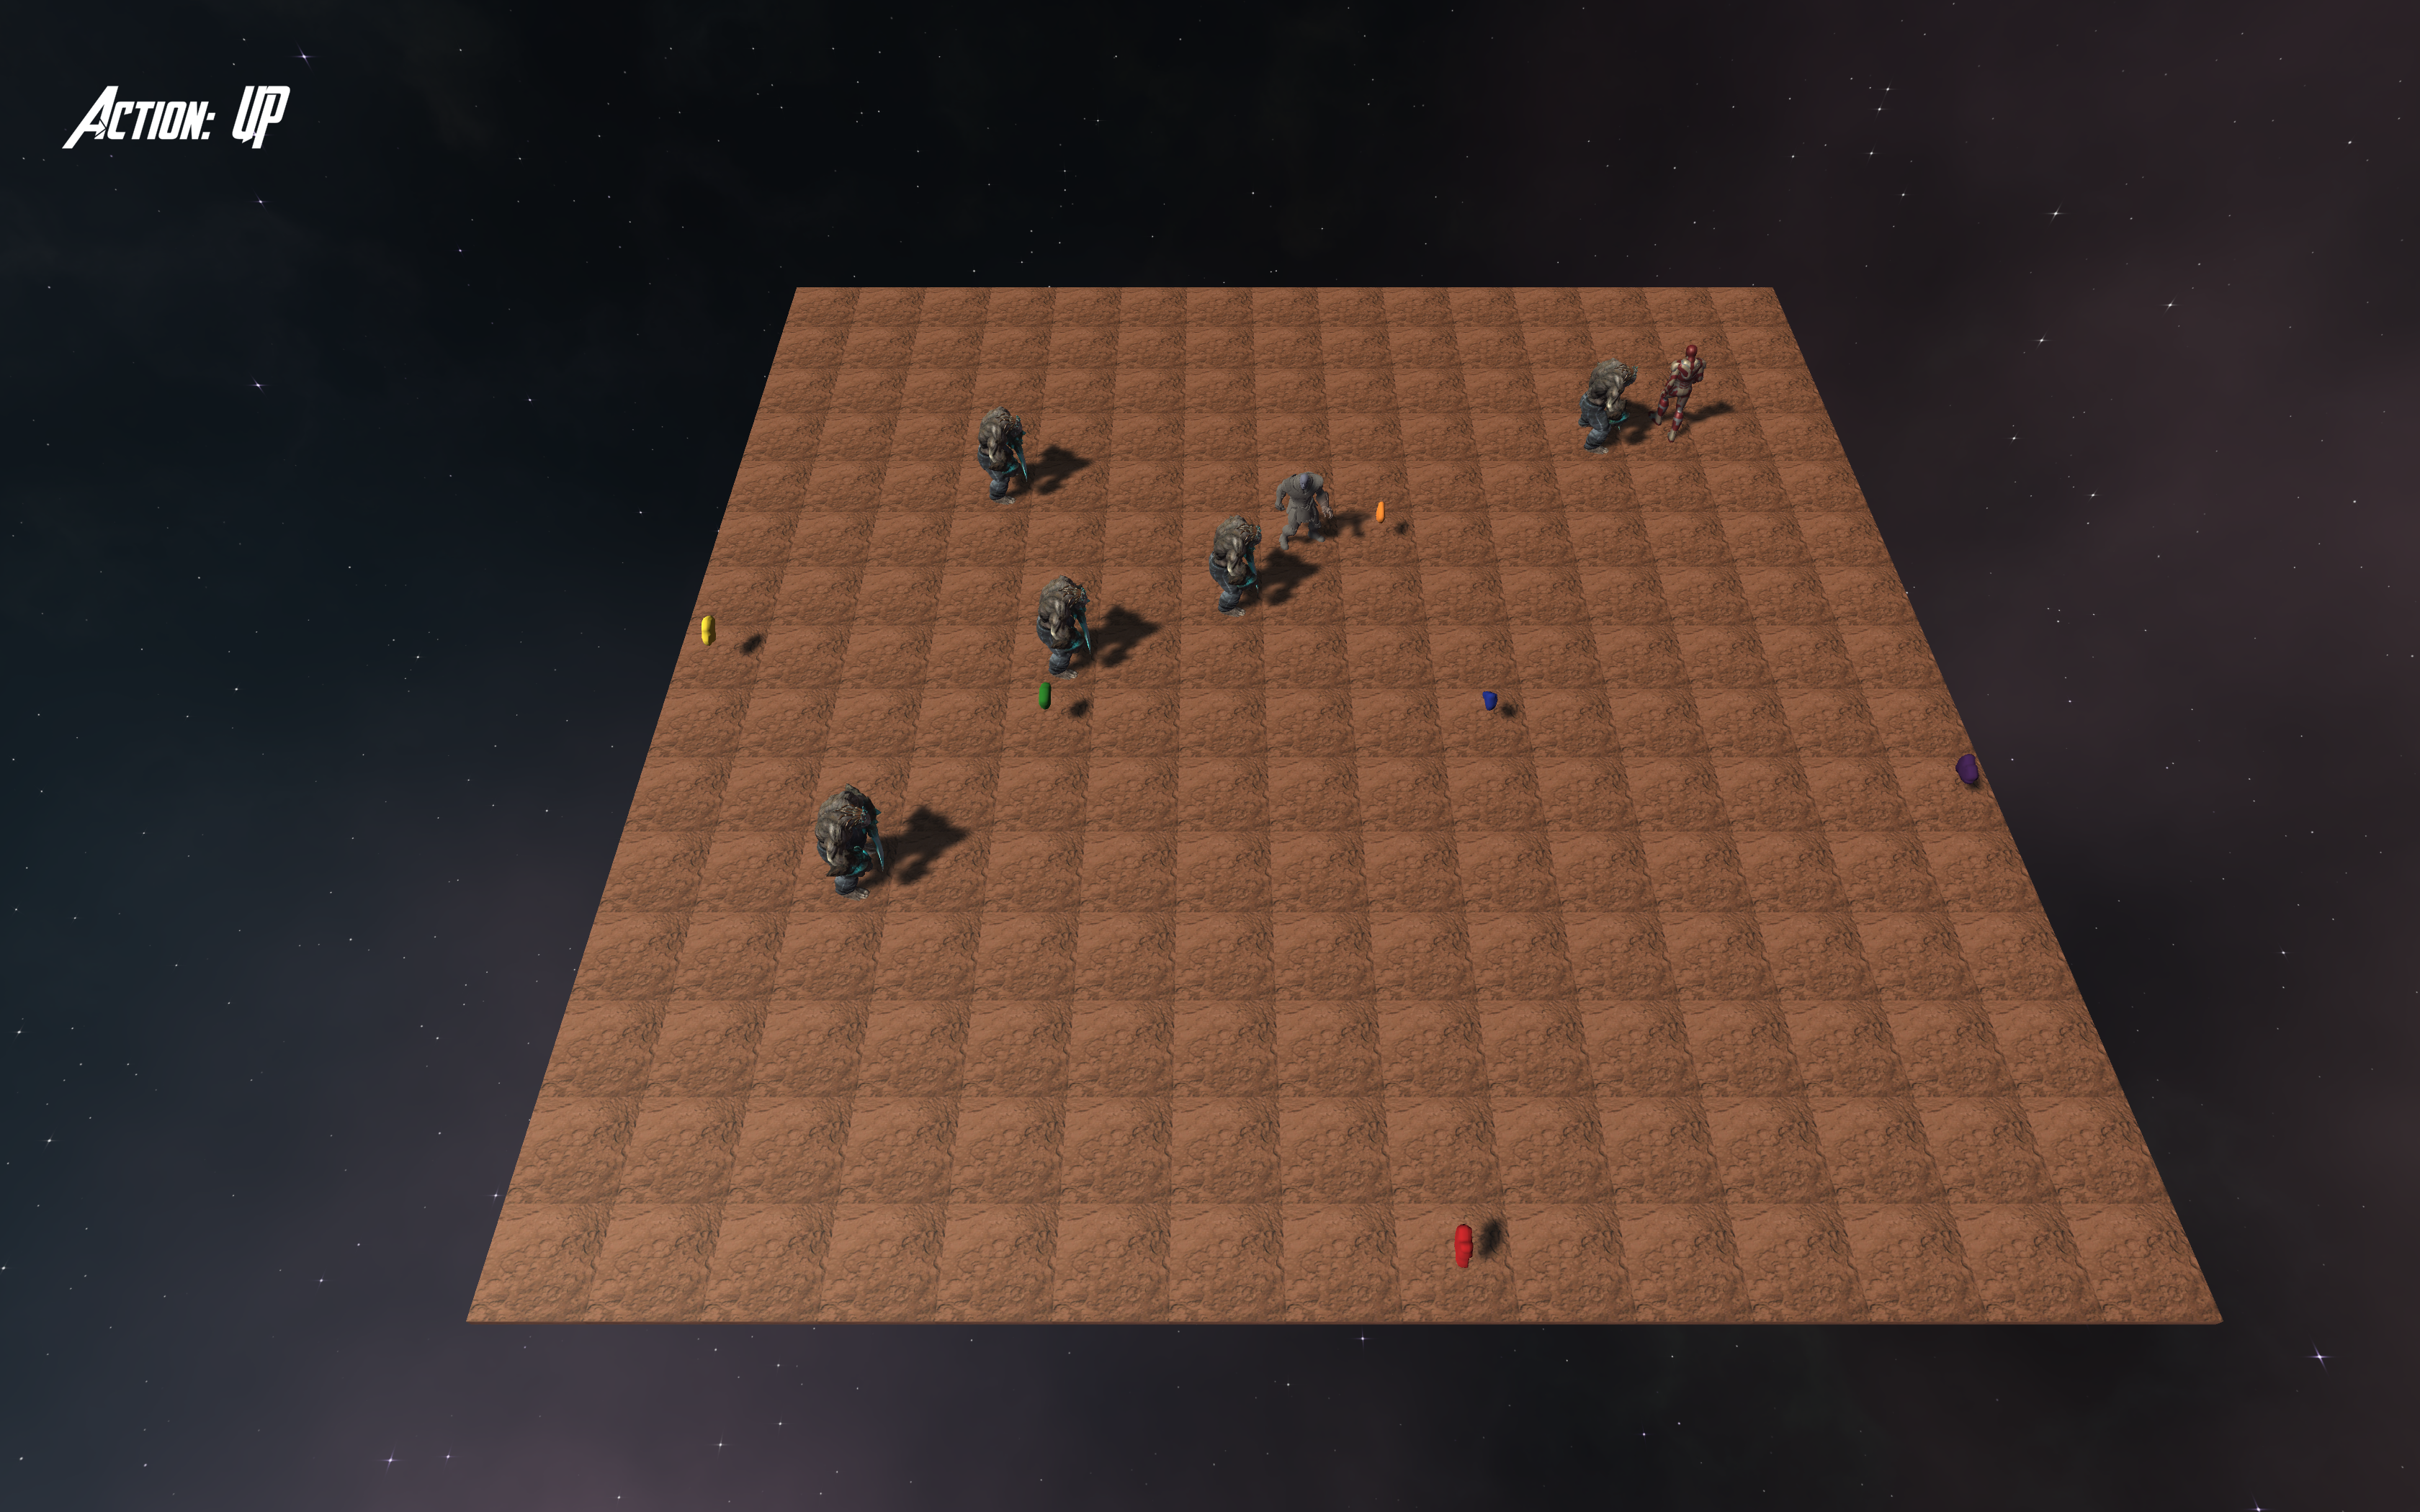
\includegraphics[width=\linewidth]{figures/endgamevisualization.png}
  \caption{Unity EndGame Visualization}
  \label{fig:endgamevisualization}
\end{figure}

\clearpage

\subsection{Universe (7 x 7)}
The first running example is a (7 x 7) universe are shown in the figure~\ref{fig:7by7}. A detailed results are found the the table~\ref{tab:7by7} below which should the performance of each strategy along with the estimated time for solving the problem and the total expanded nodes in each algorithm.

\begin{figure}[!hpt]
  \centering
  \includegraphics[width=\linewidth]{figures/7by7.png}
  \caption{The terminal representation for 7x7 universe}
  \label{fig:7by7}
\end{figure}


\begin{table}[!hpt]
  \centering
  \begin{tabular}{|c|c|c|c|c|c|c|}
  \hline
  \cellcolor[HTML]{9B9B9B}\textit{\textbf{7 x 7}} & \textbf{Expanded Nodes} & \textbf{Depth} & \textbf{Path Cost} & \textbf{Estimates Time} & \textbf{Completeness} & \textbf{Optimality} \\ \hline
  \textbf{BFS}                                    & 108896                  & 28             & 38                 & 2s 868ms     & True & False           \\ \hline
  \textbf{DFS}                                    & 1351                    & \cellcolor[HTML]{ffcccb}128            & 92                 & 87ms         & True & False           \\ \hline
  \textbf{IDS}                                    & \cellcolor[HTML]{ffcccb}496932                  & 47             & 34                 & 4s 430ms     & True & False           \\ \hline
  \textbf{UCS}                                    & 62682                   & 43             & 32                 & 591 ms       & True & True           \\ \hline
  \textbf{GR1}                                    & 316                     & 46             & 44                 & \cellcolor[HTML]{90ee90}6 ms         & True & False           \\ \hline
  \textbf{GR2}                                    & 226                     & 56             & 65                 & 24 ms        & True & False           \\ \hline
  \textbf{AS1}                                    & 35632                   & 61             & 32                 & 626 ms       & True & True           \\ \hline
  \textbf{AS2}                                    & 33532                   & 56             & 31                 & 2s 105ms     & True & True           \\ \hline
  \end{tabular}
  \caption{7 x 7 Universe Comparison}
  \label{tab:7by7}
  \end{table}

The table above summaries all the running strategies on the 7 by 7 universe where we can notice that depth first strategy reaches the deepest level in the search tree and iterative deepening search has the most number of expanded nodes and it's execution time is the highest. The fastest running algorithm was greedy search strategy using the first heuristic function and the most optimized solution is from A star algorithm using the second heuristic function.

  \clearpage

\subsection{Universe (15 x 15)}
The second running example is a (15 x 15) universe are shown in the figure~\ref{fig:15by15}. A detailed results are found the the table~\ref{tab:15by15} below which should the performance of each strategy along with the estimated time for solving the problem and the total expanded nodes in each algorithm.

\begin{figure}[!hpt]
  \centering
  \includegraphics[width=\linewidth]{figures/15by15.png}
  \caption{The terminal representation for 15x15 universe}
  \label{fig:15by15}
\end{figure}


\begin{table}[!hpt]
  \centering
  \begin{tabular}{|c|c|c|c|c|c|c|}
  \hline
  \cellcolor[HTML]{9B9B9B}\textit{\textbf{15 x 15}} & \textbf{Expanded Nodes} & \textbf{Depth} & \textbf{Path Cost} & \textbf{Estimates Time} & \textbf{Completeness} & \textbf{Optimality} \\ \hline
  \textbf{BFS}                                      & 812811                  & 51             & 46                 & 18s 452 ms  & True & False            \\ \hline
  \textbf{DFS}                                      & 547112                  & \cellcolor[HTML]{ffcccb}511            & 90                 & 4s 96 ms    & True & False            \\ \hline
  \textbf{IDS}                                      & \cellcolor[HTML]{ffcccb}3779426                 & 136            & 37                 & 26s 757 ms  & True & False            \\ \hline
  \textbf{UCS}                                      & 295564                  & 144            & 35                 & 4s 97 ms    & True & True            \\ \hline
  \textbf{GR1}                                      & 685                     & 118            & 48                 & 56 ms       & True & False            \\ \hline
  \textbf{GR2}                                      & 685                     & 118            & 48                 & 138 ms      & True & False            \\ \hline
  \textbf{AS1}                                      & 167443                  & 224            & 35                 & 2s 262 ms   & True & True            \\ \hline
  \textbf{AS2}                                      & 131729                  & 170            & 35                 & 8s 332      & True & True            \\ \hline
  \end{tabular}
  \caption{15 x 15 Universe Comparison}
  \label{tab:15by15}
  \end{table}

The table above summaries all the running strategies on the 15 by 15 universe where we can notice that depth first strategy reaches the deepest level in the search tree and iterative deepening search has the most number of expanded nodes and it's execution time is the highest. The fastest running algorithm was greedy search strategy using the first heuristic function and the most optimized solutions are from uniform cost and A star algorithm using both heuristic function.

\section{Future Work}

This project will be extended to include reinforcement learning and logic based agents. A more generalized approaches and optimization should be added and new strategies should be testes and compared with the existing strategies. Experiments with randomization and change of actions should be done along with increasing the level of difficulty for solving the new environment.

\section{Acknowledgement}

We would like to thank our professor \textbf{\textit{Haythem Ismail}} for the interesting lectures and content we are studying and the research questions and projects that enhance our skilss and experience for building intelligent agents. A special thanks to Eng. \textbf{\textit{Nourhan Ehab}} for her amazing way of teaching and wonderful personality and all the help provided for us towards understanding how to build intelligent agents and this interesting research project.



\bibliographystyle{unsrt}  
\bibliography{references}  %%% Remove comment to use the external .bib file (using bibtex).
%%% and comment out the ``thebibliography'' section.

\end{document}
